\section{Discretization of the Unit Square}
\label{sec:discretization}

It is impossible to derive the incidence and Hodge matrices without any a priori knowledge about the geometry of the grid or cell-complex. Let us therefore first discretize the unit square $\Omega$ into a grid composed of points, lines, and planes. The outer-oriented grid shown in Figure \ref{fig:outerGrid} was constructed for $n = 3$, where $n$ denotes the number of planes in the horizontal and vertical directions. The grid has an orthogonal structure, but is not uniform. The points are distributed via cosine spacing at equal angular increments because the smallest flow features are expected to emerge in the vicinity of the walls, which justifies this particular refinement of the grid. The inner-oriented grid associated with the outer-oriented grid is constructed such that the inner-oriented points are located precisely in the center of the planes of the outer-oriented grid, see Figure \ref{fig:innerGrid}. The inner-oriented grid \emph{must} be constructed in this manner for reasons that can be found in literature \parencite{hirani2003discrete}.

\begin{figure}[p]
    \centering
    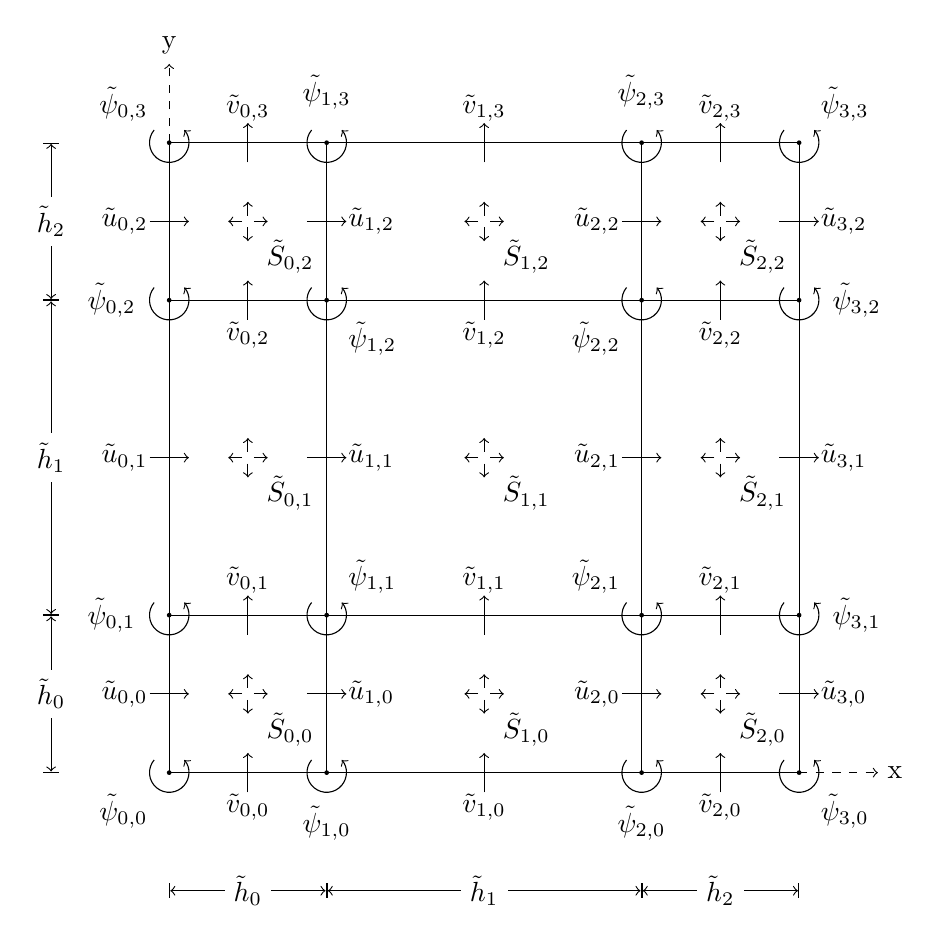
\begin{tikzpicture}
        % Draw scale
        \foreach \ia/\ib/\count in {0/2/0, 2/6/1, 6/8/2} {
            \draw [|<->|] (-1.5,\ia) -- (-1.5,\ib) node [midway,fill=white] {$\tilde{h}_\count$};
            \draw [|<->|] (\ia,-1.5) -- (\ib,-1.5) node [midway,fill=white] {$\tilde{h}_\count$};
        }
        % Draw lines
        \foreach \i in {0,2,6,8} {
            \draw (\i,0) -- (\i,8);
            \draw (0,\i) -- (8,\i);
        }
        % Draw axis
        \draw [dashed, ->] (8,0) -- (9,0) node [right] {x};
        \draw [dashed, ->] (0,8) -- (0,9) node [above] {y};
        % Four courner points
        \fill (0,0) circle (0.03) node [below left=1ex] {$\tilde{\psi}_{0,0}$};
        \fill (8,0) circle (0.03) node [below right=1ex] {$\tilde{\psi}_{3,0}$};
        \fill (8,8) circle (0.03) node [above right=1ex] {$\tilde{\psi}_{3,3}$};
        \fill (0,8) circle (0.03) node [above left=1ex] {$\tilde{\psi}_{0,3}$};
        % Bottom boundary
        \fill (2,0) circle (0.03) node [below=2ex] {$\tilde{\psi}_{1,0}$};
        \fill (6,0) circle (0.03) node [below=2ex] {$\tilde{\psi}_{2,0}$};
        % Right boundary
        \fill (8,2) circle (0.03) node [right=2ex] {$\tilde{\psi}_{3,1}$};
        \fill (8,6) circle (0.03) node [right=2ex] {$\tilde{\psi}_{3,2}$};
        % Top boundary
        \fill (6,8) circle (0.03) node [above=2ex] {$\tilde{\psi}_{2,3}$};
        \fill (2,8) circle (0.03) node [above=2ex] {$\tilde{\psi}_{1,3}$};
        % Left boundary
        \fill (0,6) circle (0.03) node [left=2ex] {$\tilde{\psi}_{0,2}$};
        \fill (0,2) circle (0.03) node [left=2ex] {$\tilde{\psi}_{0,1}$};
        % Inner points
        \fill (2,2) circle (0.03) node [above right=1ex] {$\tilde{\psi}_{1,1}$};
        \fill (6,2) circle (0.03) node [above left=1ex] {$\tilde{\psi}_{2,1}$};
        \fill (6,6) circle (0.03) node [below left=1ex] {$\tilde{\psi}_{2,2}$};
        \fill (2,6) circle (0.03) node [below right=1ex] {$\tilde{\psi}_{1,2}$};
        % Rounded arrow
        \foreach \x/\i in {0/0, 2/1, 6/2, 8/3} {
            \foreach \y/\j in {0/0, 2/1, 6/2, 8/3} {
                \draw [->] (\x,\y) ++(140:0.25) arc (-220:40:0.25);
            }
        }
        % Draw u
        \foreach \x/\i in {0/0, 6/2} {
            \foreach \y/\j in {1/0, 4/1, 7/2} {
                \draw [->] (\x-0.25,\y) -- (\x+0.25,\y);
                \node[left=1ex] at (\x,\y) {$\tilde{u}_{\i,\j}$};
            }
        }
        \foreach \x/\i in {2/1, 8/3} {
            \foreach \y/\j in {1/0, 4/1, 7/2} {
                \draw [->] (\x-0.25,\y) -- (\x+0.25,\y);
                \node[right=1ex] at (\x,\y) {$\tilde{u}_{\i,\j}$};
            }
        }
        % Draw v
        \foreach \x/\i in {0/0, 6/2} {
            \foreach \y/\j in {1/0, 4/1, 7/2} {
                \draw [->] (\y,\x-0.25) -- (\y,\x+0.25);
                \node[below=1ex] at (\y,\x) {$\tilde{v}_{\j,\i}$};
            }
        }
        \foreach \x/\i in {2/1, 8/3} {
            \foreach \y/\j in {1/0, 4/1, 7/2} {
                \draw [->] (\y,\x-0.25) -- (\y,\x+0.25);
                \node[above=1ex] at (\y,\x) {$\tilde{v}_{\j,\i}$};
            }
        }
        % Draw p
        \foreach \x/\i in {1/0, 4/1, 7/2} {
            \foreach \y/\j in {1/0, 4/1, 7/2} {
                \node[below right=0.75ex] at (\x,\y) {$\tilde{S}_{\i,\j}$};
                \draw [->] (\x+0.075,\y) -- (\x+0.25,\y);
                \draw [->] (\x-0.075,\y) -- (\x-0.25,\y);
                \draw [->] (\x,\y+0.075) -- (\x,\y+0.25);
                \draw [->] (\x,\y-0.075) -- (\x,\y-0.25);
            }
        }
    \end{tikzpicture}
    \caption{The outer-oriented grid.}
    \label{fig:outerGrid}
\end{figure}

\begin{figure}[p]
    \centering
    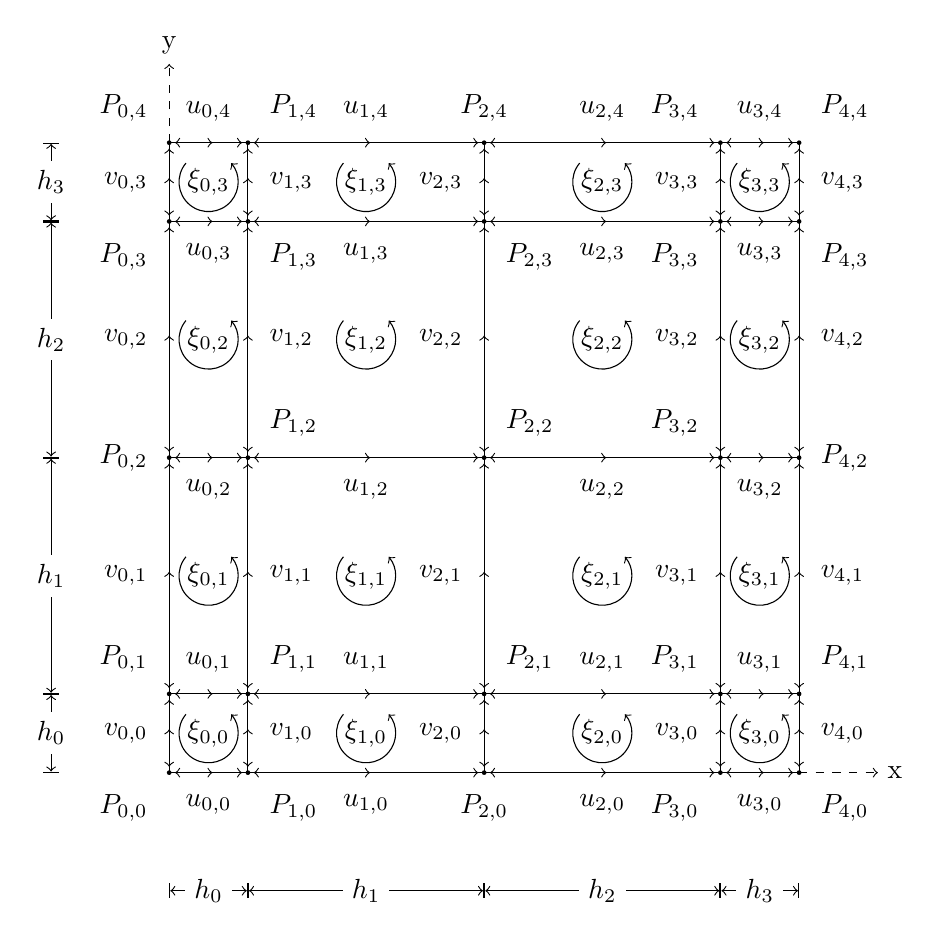
\begin{tikzpicture}
        % Draw scale
        \foreach \ia/\ib/\count in {0/1/0, 1/4/1, 4/7/2, 7/8/3} {
            \draw [|<->|] (-1.5,\ia) -- (-1.5,\ib) node [midway,fill=white] {$h_\count$};
            \draw [|<->|] (\ia,-1.5) -- (\ib,-1.5) node [midway,fill=white] {$h_\count$};
        }
        % Draw lines
        \foreach \i in {0,1,4,7,8} {
            \draw (\i,0) -- (\i,8);
            \draw (0,\i) -- (8,\i);
        }
        % Draw axis
        \draw [dashed, ->] (8,0) -- (9,0) node [right] {x};
        \draw [dashed, ->] (0,8) -- (0,9) node [above] {y};
        % Draw p
        \foreach \x/\i in {0/0, 1/1, 4/2, 7/3} {
            \foreach \y/\j in {0/0, 1/1, 4/2, 7/3, 8/4} {
                \draw [<-] (\x+0.075,\y) -- (\x+0.25,\y);
            }
        }
        \foreach \x/\i in {1/1, 4/2, 7/3, 8/4} {
            \foreach \y/\j in {0/0, 1/1, 4/2, 7/3, 8/4} {
                \draw [<-] (\x-0.075,\y) -- (\x-0.25,\y);
            }
        }
        \foreach \x/\i in {0/0, 1/1, 4/2, 7/3, 8/4} {
            \foreach \y/\j in {0/0, 1/1, 4/2, 7/3} {
                \draw [<-] (\x,\y+0.075) -- (\x,\y+0.25);
            }
        }
        \foreach \x/\i in {0/0, 1/1, 4/2, 7/3, 8/4} {
            \foreach \y/\j in {1/1, 4/2, 7/3, 8/4} {
                \draw [<-] (\x,\y-0.075) -- (\x,\y-0.25);
            }
        }
        % Four corner points
        \fill (0,0) circle (0.03) node [below left=1ex] {$P_{0,0}$};
        \fill (8,0) circle (0.03) node [below right=1ex] {$P_{4,0}$};
        \fill (8,8) circle (0.03) node [above right=1ex] {$P_{4,4}$};
        \fill (0,8) circle (0.03) node [above left=1ex] {$P_{0,4}$};
        % Bottom boundary
        \fill (1,0) circle (0.03) node [below right=1ex] {$P_{1,0}$};
        \fill (4,0) circle (0.03) node [below=1ex] {$P_{2,0}$};
        \fill (7,0) circle (0.03) node [below left=1ex] {$P_{3,0}$};
        % Right boundary
        \fill (8,1) circle (0.03) node [above right=1ex] {$P_{4,1}$};
        \fill (8,4) circle (0.03) node [right=1ex] {$P_{4,2}$};
        \fill (8,7) circle (0.03) node [below right=1ex] {$P_{4,3}$};
        % Top boundary
        \fill (7,8) circle (0.03) node [above left=1ex] {$P_{3,4}$};
        \fill (4,8) circle (0.03) node [above=1ex] {$P_{2,4}$};
        \fill (1,8) circle (0.03) node [above right=1ex] {$P_{1,4}$};
        % Left boundary
        \fill (0,7) circle (0.03) node [below left=1ex] {$P_{0,3}$};
        \fill (0,4) circle (0.03) node [left=1ex] {$P_{0,2}$};
        \fill (0,1) circle (0.03) node [above left=1ex] {$P_{0,1}$};
        % Four interior corners
        \fill (1,1) circle (0.03) node [above right=1ex] {$P_{1,1}$};
        \fill (7,1) circle (0.03) node [above left=1ex] {$P_{3,1}$};
        \fill (7,7) circle (0.03) node [below left=1ex] {$P_{3,3}$};
        \fill (1,7) circle (0.03) node [below right=1ex] {$P_{1,3}$};
        % Five remaining interior points
        \fill (4,1) circle (0.03) node [above right=1ex] {$P_{2,1}$};
        \fill (7,4) circle (0.03) node [above left=1ex] {$P_{3,2}$};
        \fill (4,7) circle (0.03) node [below right=1ex] {$P_{2,3}$};
        \fill (1,4) circle (0.03) node [above right=1ex] {$P_{1,2}$};
        \fill (4,4) circle (0.03) node [above right=1ex] {$P_{2,2}$};
        % Draw v
        \foreach \x/\i in {0/0, 4/2, 7/3} {
            \foreach \y/\j in {0.5/0, 2.5/1, 5.5/2, 7.5/3} {
                \draw [->] (\x,\y) -- (\x,\y+0.05);
                \node[left=1ex] at (\x,\y) {$v_{\i,\j}$};
            }
        }
        \foreach \x/\i in {1/1, 8/4} {
            \foreach \y/\j in {0.5/0, 2.5/1, 5.5/2, 7.5/3} {
                \draw [->] (\x,\y) -- (\x,\y+0.05);
                \node[right=1ex] at (\x,\y) {$v_{\i,\j}$};
            }
        }
        % Draw u
        \foreach \x/\i in {0/0, 4/2, 7/3} {
            \foreach \y/\j in {0.5/0, 2.5/1, 5.5/2, 7.5/3} {
                \draw [->] (\y,\x) -- (\y+0.05,\x);
                \node[below=1ex] at (\y,\x) {$u_{\j,\i}$};
            }
        }
        \foreach \x/\i in {1/1, 8/4} {
            \foreach \y/\j in {0.5/0, 2.5/1, 5.5/2, 7.5/3} {
                \draw [->] (\y,\x) -- (\y+0.05,\x);
                \node[above=1ex] at (\y,\x) {$u_{\j,\i}$};
            }
        }
        % Draw xi
        \foreach \x/\i in {0.5/0, 2.5/1, 5.5/2, 7.5/3} {
            \foreach \y/\j in {0.5/0, 2.5/1, 5.5/2, 7.5/3} {
                \draw [->] (\x,\y) ++(140:0.375) arc (-220:40:0.375);
                \node at (\x,\y) {$\xi_{\i,\j}$};
            }
        }
    \end{tikzpicture}
    \caption{The inner-oriented grid.}
    \label{fig:innerGrid}
\end{figure}

\section{Physical Representation}

We briefly digress here to summarize the physical interpretation of the $k$-cells that compose the inner and outer oriented grids. The orientation of the outer-oriented planes $\tilde{S}_{i,j}$ is source-like, as indicated by the outward pointing arrows. That is, an outflow is considered positive and an inflow is considered negative. The outer-oriented line segments $\tilde{u}_{i,j}$ and $\tilde{v}_{i,j}$ represent flux in the form:
\begin{flalign}
    \stepcounter{equation}
    \tag{{\theequation}a}
    & & \tilde{u}_{i,j} = \int_{y_{i,j}}^{y_{i,j+1}} \mathbf{u} \cdot  \mathbf{\hat{n}} \, dy && \\
    \tag{{\theequation}b}
    &\text{and}& \tilde{v}_{i,j} = \int_{x_{i,j}}^{x_{i+1,j}} \mathbf{u} \cdot \mathbf{\hat{n}} \, dx &&
\end{flalign}
where $\mathbf{\hat{n}}$ denotes the normal vector along the line segment. (\textit{Note:} it is important to remember that all physical quantities are still dimensionless.) A rightward and upward flux is considered positive, as indicated by the arrows through the line segments in Figure \ref{fig:outerGrid}. If outer-oriented 1-cochains represent flux, then outer-oriented 0-cochains must represent samples of the the continuous stream function and outer-oriented 2-cochains must represent the rate of mass production within the plane on which they are defined.

The inner-oriented line segments $u_{i,j}$ and $v_{i,j}$ represent circulation: 
\begin{flalign}
    \stepcounter{equation}
    \tag{{\theequation}a}
    & & u_{i,j} = \int_{x_{i,j}}^{x_{i,j+1}} \mathbf{u} \cdot  \mathbf{\hat{t}} \, dx && \\
    \tag{{\theequation}b}
    &\text{and}& v_{i,j} = \int_{y_{i,j}}^{y_{i+1,j}} \mathbf{u} \cdot \mathbf{\hat{t}} \, dy &&
\end{flalign}
where $\mathbf{\hat{t}}$ denotes the tangent vector along the line segment.
As discussed in the preceding section, application of the integrated curl operator on a velocity field yields vorticity, assuming that the surfaces are infinitesimal. The inner-oriented 2-cochains $\xi_{(i,j)}$ do therefore represent vorticity and the inner-oriented 0-cochains $P_{i,j}$ represent total pressure. Notice that the orientation of the inner-oriented 0-cochains $P_{i,j}$ is sink-like, as indicated by the inward pointing arrows.

We have constructed the inner and outer oriented grid and we have established what the $k$-cells physically represent. The double DeRham complex can be updated incorporating the physical quantities:
\begin{equation}
    \label{eq:rham1}
    \begin{gathered}
        \xymatrix@=20ex{
            \mathbf{P}^{(0)} \ar[r]^{\mathbb{E}^{(1,0)}}_{\text{grad}} \ar@<1ex>[d]^{\mathbb{H}^{(\tilde{2},0)}} & \mathbf{u}^{(1)} \ar[r]^{\mathbb{E}^{(2,1)}}_{\text{curl}} \ar@<1ex>[d]^{\mathbb{H}^{(\tilde{1},1)}} & \mathbf{\xi}^{(2)} \ar@<1ex>[d]^{\mathbb{H}^{(\tilde{0},2)}} \\
            \mathbf{\tilde{S}}^{(2)} \ar@<1ex>[u]^{\mathbb{H}^{(0,\tilde{2})}} & \mathbf{\tilde{u}}^{(1)} \ar[l]_{\tilde{\mathbb{E}}^{(2, 1)}}^{\text{curl}} \ar@<1ex>[u]^{\mathbb{H}^{(1,\tilde{1})}} & \mathbf{\tilde{\psi}}^{(0)} \ar[l]_{\tilde{\mathbb{E}}^{(1,0)}}^{\text{grad}} \ar@<1ex>[u]^{\mathbb{H}^{(2,\tilde{0})}}
        }
    \end{gathered}
\end{equation}

(\textit{Note:} The variables in Equation \eqref{eq:rham1} are written in boldface because their numerical values are typically stored in an array (i.e., a vector) on a computer. However, the physical quantities $P$ and $\mathbf{\tilde{\psi}}$ remain scalar quantities and should \emph{not} be seen as vector quantities.)
